\documentclass[12pt,a4paper]{report}

% --- Page layout (IIT Roorkee template: A4, 1 inch margins, 1.5 spacing) ---
\usepackage[a4paper,left=1in,right=1in,top=1in,bottom=1in]{geometry}
\usepackage[T1]{fontenc}
\usepackage{mathptmx}
\usepackage{microtype}
\usepackage{setspace}
\onehalfspacing
\usepackage{etoolbox}
\AtBeginEnvironment{table}{\singlespacing\small}
\AtBeginEnvironment{figure}{\singlespacing\small}
\usepackage{amsmath,amssymb}
\usepackage{booktabs,array,tabularx,multirow}
\usepackage{graphicx}
\usepackage{xcolor}
\usepackage{tikz}
\usetikzlibrary{arrows.meta,positioning,calc}
\usepackage{pgfplots}
\pgfplotsset{compat=1.16}
\usepackage{enumitem}
\usepackage{float}
\usepackage{caption}
\usepackage{titlesec}
\usepackage{chngcntr}
\usepackage{hyperref}

\hypersetup{colorlinks=true,linkcolor=black,urlcolor=blue!50!black,citecolor=black}
\setlist{itemsep=1pt,topsep=2pt,parsep=0pt}
\captionsetup{font=small,labelfont=bf,skip=4pt}
\renewcommand{\arraystretch}{1.1}
\setlength{\parindent}{0pt}
\setlength{\parskip}{5pt}
\setlength{\textfloatsep}{8pt}
\setlength{\intextsep}{8pt}

\counterwithout{table}{chapter}
\counterwithout{figure}{chapter}
\counterwithout{equation}{chapter}

\titleformat{\chapter}[block]{\centering\bfseries\fontsize{16}{20}\selectfont}{Chapter \thechapter:\ }{0pt}{}
\titlespacing*{\chapter}{0pt}{-20pt}{10pt}
\titleformat{\section}{\bfseries\fontsize{14}{17}\selectfont}{\thesection}{0.6em}{}
\titlespacing*{\section}{0pt}{8pt}{2pt}
\titleformat{\subsection}{\bfseries\fontsize{12}{15}\selectfont}{\thesubsection}{0.6em}{}
\titlespacing*{\subsection}{0pt}{6pt}{2pt}
\setcounter{secnumdepth}{2}
\setcounter{tocdepth}{1}
\renewcommand{\bibname}{References}

\newcommand{\code}[1]{\texttt{#1}}
\newcommand{\est}{\textsuperscript{$\dagger$}}
\definecolor{cA}{RGB}{70,110,170}
\definecolor{cB}{RGB}{210,120,60}
\newcommand{\frontchapter}[1]{\chapter*{#1}\addcontentsline{toc}{chapter}{#1}}

\begin{document}

% ======================= COVER =======================
\begin{titlepage}
\centering
\singlespacing
{\bfseries\fontsize{18}{22}\selectfont ANALYSIS AND OPTIMIZATION OF THE HARDWARE IMPLEMENTATION OF CRYSTALS-DILITHIUM\par}
\vspace{10pt}
{\itshape A PROJECT REPORT\par}
\vspace{10pt}
{\itshape Submitted by\par}
{\bfseries\fontsize{14}{17}\selectfont Arjun Ganesh (23114009), Atharv Bachawar (23114014)\par}
\vspace{10pt}
{\itshape for the fulfillment\par}
{\itshape of\par}
{\bfseries\fontsize{15}{18}\selectfont CSP-400A: B.Tech. Project\par}
\vspace{10pt}
{\itshape Under the guidance of\par}
{\bfseries\fontsize{14}{17}\selectfont Dr. Rajat Sadhukhan\par}
\vspace{12pt}
\IfFileExists{iitr_logo.jpeg}{
\includegraphics[width=4.6cm]{iitr_logo.jpeg}}{\fbox{\parbox[c][3cm][c]{4.6cm}{\centering\small [place iitr\_logo.jpeg\\in this folder]}}}\par
\vspace{8pt}
{\bfseries\fontsize{14}{17}\selectfont DEPARTMENT OF COMPUTER SCIENCE AND ENGINEERING\par}
{\bfseries\fontsize{14}{17}\selectfont INDIAN INSTITUTE OF TECHNOLOGY ROORKEE\par}
{\bfseries\fontsize{14}{17}\selectfont ROORKEE-247667\par}
{\bfseries\fontsize{14}{17}\selectfont 2026 - 2027\par}
\thispagestyle{empty}
\end{titlepage}

\pagenumbering{arabic}
\setcounter{page}{1}

\frontchapter{Acknowledgement}
We would like to express our sincere gratitude to our supervisor, \textbf{Dr.\ Rajat Sadhukhan} for his guidance, encouragement and valuable feedback throughout this project.

We also thank the authors of the open-source GMUCERG/Dilithium repository, whose publicly available design made this study possible, and the Department of Computer Science and Engineering, IIT Roorkee, for providing the opportunity to carry out this work as part of the course CSP-400A: B.Tech.\ Project.

\vspace{12pt}
\begin{flushright}
\textbf{Arjun Ganesh (23114009)}\\
\textbf{Atharv Bachawar (23114014)}
\end{flushright}

\frontchapter{Declaration}
We declare that this written submission represents our ideas in our own words, and where others' ideas or words have been included, we have adequately cited and referenced the original sources. We also declare that we have adhered to all principles of academic honesty and integrity and have not misrepresented or fabricated any idea, data, fact or source in our submission.

\vspace{12pt}
Place: Roorkee\\
Date: 24 November 2026

\begin{flushright}
\textbf{Arjun Ganesh (23114009)}\\
\textbf{Atharv Bachawar (23114014)}
\end{flushright}

\frontchapter{Abstract}
This report studies the open-source repository \texttt{GMUCERG/Dilithium}, an FPGA implementation of the CRYSTALS-Dilithium signature scheme in Verilog and VHDL, with C++ models of its number-theoretic transform (NTT) unit. We describe its core modules, derive its time, space and hardware complexity from the source code, and propose six optimizations, each tied to evidence in the code.

 Combined, the optimizations are projected to reduce expected signing latency by 24-37\,\%, key generation by 22-24\,\% and verification by 37-39\,\%, while reducing LUT and FF use and leaving DSP and BRAM counts unchanged.

Baseline figures come from the authors' publications. Our first-order cycle model is calibrated on them, so its agreement with the published signing latency (within 0.3\,\%) is a consistency check, not independent validation.

\renewcommand{\contentsname}{Table of Contents}
\tableofcontents

% ======================= 1 =======================
\chapter{Introduction}
% =================================================
CRYSTALS-Dilithium is a lattice-based signature scheme based on Module-LWE and Module-SIS. NIST selected it for standardization and specified it as ML-DSA in FIPS~204~\cite{fips204}. The repository analysed here, \texttt{GMUCERG/Dilithium} (commit \texttt{f929599})~\cite{repo}, accompanies the paper of Beckwith, Nguyen and Gaj~\cite{beckwith2021}.

\section{Objective}
The project (i)~explains the repository and its core modules; (ii)~derives the time, space and hardware complexity of the design from its source; (iii)~identifies optimizations that act on real bottlenecks visible in the code and estimates their effect; and (iv)~states the projected complexity of the optimized design. The optimizations are proposals for future implementation.

\section{Motivation}
Efficient hardware for a standardized post-quantum signature matters. Signing is a rejection-sampling loop with 3.85 to 5.10 expected attempts, so average signing latency is 2.3 to 3 times the best case (Table~\ref{tab:perf}). Waste inside the loop is paid on every attempt, which makes it the natural place to look for savings. A later open-source ML-DSA design is also built on this code base~\cite{norga2026}.

\section{Problem Statement and Constraints}
Given the GMU-CERG hardware implementation, explain its modules, derive its complexity, find optimizations and quantify them, and state the optimized complexity. We read the RTL and C++ sources, ran the repository's C++ NTT models, and built an analytical cycle model (Section~\ref{sec:model}).

The RTL implements the \emph{Round~3} version of Dilithium (for example $\gamma_2=95232$ at level~2), which differs from FIPS~204 in several details. The design is therefore not directly usable for ML-DSA interoperability.

\section{Organization}
Chapter~2 reviews the scheme and prior work, Chapter~3 describes the architecture, complexity and cycle model, Chapter~4 identifies bottlenecks and describes the optimizations, Chapter~5 gives results, and Chapter~6 concludes.

% ======================= 2 =======================
\chapter{Literature Survey}
% =================================================
\section{Dilithium and the Round-3 Specification}
Dilithium was introduced by Ducas et al.~\cite{spec} and follows the ``Fiat-Shamir with aborts'' paradigm of Lyubashevsky~\cite{lyubashevsky2009}: the signer samples a fresh mask, computes a response and \emph{rejects} the attempt if it could leak the secret. This loop causes the variable signing time. The repository implements the Round-3 specification; NIST later standardized a modified version as ML-DSA~\cite{fips204}.

\section{Algorithmic Background}
Polynomials live in $R_q=\mathbb{Z}_q[X]/(X^{256}+1)$ with $q=8380417=2^{23}-2^{13}+1$, and multiplication uses the NTT. Table~\ref{tab:params} lists the parameters the RTL selects through its \code{sec\_lvl} input.

\begin{table}[H]
\centering
\caption{Round-3 parameter sets supported by the design.}\label{tab:params}
\begin{tabular}{@{}lcccccccc@{}}
\toprule
Level & $K$ & $L$ & $\eta$ & $\tau$ & $\gamma_1$ & $\gamma_2$ & $\beta$ & $\omega$\\
\midrule
2 & 4 & 4 & 2 & 39 & $2^{17}$ & 95232  & 78  & 80\\
3 & 6 & 5 & 4 & 49 & $2^{19}$ & 261888 & 196 & 55\\
5 & 8 & 7 & 2 & 60 & $2^{19}$ & 261888 & 120 & 75\\
\bottomrule
\end{tabular}
\end{table}

\paragraph{Operations.}
\emph{Key generation} expands $\mathbf{A}\in R_q^{K\times L}$ from a seed $\rho$, samples short secrets $\mathbf{s}_1,\mathbf{s}_2$, computes $\mathbf{t}=\mathbf{A}\mathbf{s}_1+\mathbf{s}_2$ and splits it into $(\mathbf{t}_1,\mathbf{t}_0)$. \emph{Signing} loops: sample a mask $\mathbf{y}$, compute $\mathbf{w}=\mathbf{A}\mathbf{y}$, decompose it, hash $\mathbf{w}_1$ with the message to get a challenge $c$, form $\mathbf{z}=\mathbf{y}+c\mathbf{s}_1$, and reject unless several norm and hint checks pass. \emph{Verification} computes $\mathbf{A}\mathbf{z}-c\mathbf{t}_1 2^d$, applies the hint, re-derives the challenge and compares. It is a single pass.

\paragraph{Rejection probability.}
An attempt needs $\|\mathbf{z}\|_\infty<\gamma_1-\beta$ and $\|\mathbf{r}_0\|_\infty<\gamma_2-\beta$, plus later conditions on $c\mathbf{t}_0$ and the hint count. Treating coefficients as independent,
\begin{equation}
  p_z\approx e^{-256L\beta/\gamma_1},\quad
  p_r\approx e^{-256K\beta/\gamma_2},\quad
  \mathbb{E}[R]\approx \frac{1}{p_zp_r}.
  \label{eq:rep}
\end{equation}
This gives 4.25, 5.095 and 3.85 attempts at levels 2, 3 and 5; the specification states 4.25, 5.1 and 3.85. We use 5.10 for level~3 throughout. Table~\ref{tab:prob} gives the probabilities that an attempt stops at each check.

\begin{table}[H]
\centering
\caption{Success probabilities and stopping points per attempt.}\label{tab:prob}
\begin{tabular}{@{}lccccccc@{}}
\toprule
Level & $p_z$ & $p_r$ & $p_zp_r$ & $\mathbb{E}[R]$ & stop at $\mathbf{z}$ & stop at $\mathbf{r}_0$ & reach $c\mathbf{t}_0$\\
\midrule
2 & 0.544 & 0.432 & 0.235 & 4.25 & 45.6\,\% & 30.9\,\% & 23.5\,\%\\
3 & 0.620 & 0.317 & 0.196 & 5.10 & 38.0\,\% & 42.3\,\% & 19.6\,\%\\
5 & 0.664 & 0.391 & 0.260 & 3.85 & 33.6\,\% & 40.4\,\% & 26.0\,\%\\
\bottomrule
\end{tabular}
\end{table}

\section{Prior Hardware Work and the Repository}
Land, Sasdrich and G\"uneysu~\cite{land2021} and Zhao et al.~\cite{zhao2022} proposed other Dilithium hardware designs. Beckwith, Nguyen and Gaj~\cite{beckwith2021} present a high-performance core supporting all three levels, with results in a later paper~\cite{beckwith2022}. We study this one because its source is public and complete. We did not survey the others exhaustively and make no claim about whether they use the changes proposed here.

The design relies on pipelined butterflies for the NTT, Barrett reduction~\cite{barrett1986} (Montgomery reduction~\cite{montgomery1985} is the usual alternative) and Keccak-based SHAKE~\cite{fips202}.

The repository~\cite{repo} contains about 10{,}900 lines of RTL (Verilog, plus a VHDL Keccak core), three testbenches (1{,}850 lines) with known-answer test (KAT) vectors for all levels, C++ models of the NTT in plain and hardware-style form, and the twiddle table. Because of the VHDL core, mixed-language simulation is needed. The testbenches print the cycle counts used in the authors' paper.

% ======================= 3 =======================
\chapter{Methodology}
% =================================================
\section{Method of Study}
We (1)~read the RTL and C++ sources; (2)~ran the C++ NTT models to check structural claims; (3)~derived operation counts, cycles, memory and area from the code and the authors' reported figures; (4)~built a first-order cycle model of the state machines; and (5)~used the model to find bottlenecks and size each optimization.

\section{Architecture and Core Modules}
Figure~\ref{fig:arch} shows the structure. The top module \code{combined\_top} (2{,}553 lines) holds three finite-state machines, seven dual-port RAMs, three Keccak cores, the samplers, and two polynomial ``operators'' (\code{NUM\_OPERATORS = 2}). Data moves over a 64-bit valid/ready interface.

\begin{figure}[H]
\centering
\resizebox{0.92\textwidth}{!}{\begin{tikzpicture}[
  font=\small,
  box/.style={draw,rounded corners=2pt,minimum height=8mm,minimum width=34mm,align=center,fill=gray!8},
  arr/.style={-{Stealth[length=2mm]},thick},
  arrb/.style={{Stealth[length=2mm]}-{Stealth[length=2mm]},thick}]
  \node[box] (io)  at (0,0)    {64-bit I/O\\valid/ready};
  \node[box] (dec) at (0,-1.9) {Decoder /\\Encoder};
  \node[box] (fsm) at (0,-3.8) {FSM0 / FSM1 / FSM2\\(control)};
  \node[box] (hint) at (5.6,0)    {Decomposer, MakeHint,\\UseHint, norm check};
  \node[box] (ram)  at (5.6,-1.9) {7 BRAMs, 96-bit words\\(4 coefficients each)};
  \node[box] (op)   at (5.6,-3.8) {2 $\times$ operator: address unit,\\twiddle ROM, 2$\times$2 butterflies, FIFO};
  \node[box] (smp) at (11.2,-1.9) {SampleA, S, Y, C\\(rejection sampling)};
  \node[box] (kec) at (11.2,-3.8) {3 $\times$ Keccak\\(SHAKE128/256)};
  \draw[arr] (io) - (dec);
  \draw[arr] (dec) - (ram);
  \draw[arrb] (ram) - (hint);
  \draw[arrb] (ram) - (op);
  \draw[arr] (fsm) - (op);
  \draw[arrb] (smp) - (ram);
  \draw[arrb] (smp) - (kec);
\end{tikzpicture}}
\caption{Simplified block diagram of \code{combined\_top}.}\label{fig:arch}
\end{figure}

\paragraph{Control.}
Key generation (10 states) and verification (14 states) are strictly sequential chains, and only operator~0 is ever driven in them; operator~1 appears only in signing branches (we checked every use of \code{op[1]}). Signing uses three concurrent machines. FSM0 loads the key and transforms $\mathbf{s}_1,\mathbf{s}_2,\mathbf{t}_0$. FSM1 prepares the \emph{next} attempt ($\mathbf{y}$, its transform, the product with $\mathbf{A}$, the inverse transform to $\mathbf{w}$) on operator~0. FSM2 finishes the \emph{current} attempt on operator~1: decomposition, challenge, the products with $\mathbf{s}_1,\mathbf{s}_2,\mathbf{t}_0$, norm checks and hint creation. Consecutive attempts therefore overlap.

\paragraph{Memory.}
Each 96-bit RAM word holds four 24-bit coefficients, so a polynomial takes 64 words. \code{BRAM\_0} (64 polynomials) holds $\mathbf{A}$; \code{BRAM\_1}-\code{BRAM\_6} (16 polynomials each) hold the other vectors. This is 160 slots (120\,KiB), sized for level~5. All RAM ports are wired by large per-state \code{case} statements in the top module, with no central arbiter.

\paragraph{Other modules.}
SampleA, S, Y and C turn Keccak output into coefficients by rejection sampling; the decomposer, MakeHint, UseHint and norm-check blocks handle the rejection tests. Core~0 and~1 serve SampleA in parallel, and core~2 serves everything else. A SHAKE128 polynomial needs about 4.6 blocks (five permutations); we assume one Keccak round per clock, i.e.\ 24 cycles per permutation, without tracing the round datapath.

\section{The NTT Unit}
\code{butterfly2x2} chains two layers of two butterflies, so one pass over the 64 words performs two layers on all 256 coefficients and eight layers take four passes. A four-way FIFO transposes data between layers. The forward transform is decimation in frequency and the inverse is decimation in time, so no bit reversal is needed. Each butterfly multiplies by a twiddle factor (24$\times$24 bits) and reduces with a three-stage Barrett reducer built from shift-and-add trees, so only the data multiplication uses DSPs. The inverse transform halves values at each layer, which folds in the $256^{-1}$ factor. The same four butterflies also do pointwise multiply-accumulate, addition and subtraction.

\section{Rejection Handling in Signing}\label{sec:reject}
The norm checks see data as it is written to memory, gated to the last inverse-transform pass. A sticky flag \code{norm\_rejected} records any violation, but it is only \emph{read} at the end of \code{FSM2\_MAKEHINT} (\code{combined\_top.v}, lines 2217-2221). Until then FSM2 advances unconditionally through all stages. This is the root of optimization~O1.

\paragraph{Caveat.}
This rests on our reading of the control code. Before implementing O1, confirm by text search for all uses of \code{norm\_rejected} and by waveform inspection of a rejected attempt that no other path already short-circuits the stages.

\paragraph{Other code observations.}
\code{operation\_module.v} (lines 83, 85) loads the twiddle ROM from an absolute Windows path, which blocks building elsewhere. In \code{combined\_top.v} (line 2259) the reset branch assigns \code{cstate1 <= FSM2\_STALL;} where \code{cstate2} was almost certainly intended; it is harmless only because both constants equal 0.

\section{Complexity Analysis}
Let $N=256$ and $P=4$ butterflies in parallel. An NTT needs $\tfrac N2\log_2N=1024$ butterflies, $\Theta(N\log N)$; a pointwise product needs $N$ multiplications. The ideal latencies are $1024/P=256$ cycles per NTT and $N/4=64$ per pointwise pass. Table~\ref{tab:opcount} counts polynomial primitives; each operation is dominated by transforms, $\Theta\big((K{+}L)N\log N+KLN\big)$ per pass, and signing multiplies this by the constant $\mathbb{E}[R]$.

\begin{table}[H]
\centering
\caption{Polynomial-primitive counts (signing per attempt; one-off signing setup needs $L+2K$ transforms).}\label{tab:opcount}
\begin{tabular}{@{}lcc@{}}
\toprule
Operation & Transforms & Pointwise products\\
\midrule
Key generation & $L+K$ & $KL$ (+$K$ additions)\\
Signing, per attempt & $2L+3K+1$ & $KL+L+2K$\\
Verification & $L+2K+1$ & $KL+K$ (+$K$ subtractions)\\
Sign attempt, levels 2 / 3 / 5 & 21 / 29 / 39 & 28 / 47 / 79\\
\bottomrule
\end{tabular}
\end{table}

\paragraph{Cycle-level time.}
Four passes of 64 words give 256 streaming cycles. Two additions are visible in \code{operation\_module.v}: inter-pass pauses of 7 (forward) or 5 (inverse) cycles at each of three boundaries, i.e.\ 21 and 15 cycles, and a pipeline fill/drain of about 23 cycles (the write-back address shift register is about 22 stages deep; we obtained 23 by subtracting the other terms from the reported totals). This gives 300 cycles forward and 294 inverse, the authors' reported values; since 23 was derived from them, the match holds by construction. A pointwise pass takes about $T_p=72$ cycles.

\paragraph{Space.}
The polynomials live during signing are $\mathbf{A}$ ($KL$), $\hat{\mathbf{y}},\mathbf{z},\hat{\mathbf{s}}_1$ ($L$ each), $\hat{\mathbf{s}}_2,\hat{\mathbf{t}}_0,\mathbf{w},c\mathbf{s}_2,c\mathbf{t}_0$ ($K$ each) and $\hat c$:
\begin{equation}
  S_{\text{poly}}=KL+3L+5K+1=49,\;76,\;118\ \text{polynomials}=\Theta\big((KL+K+L)N\big)\text{ coefficients.}
  \label{eq:space}
\end{equation}

\paragraph{Hardware.}
The datapath is $\Theta(P)$ butterflies (one multiplier, one reducer, two adders each); memory is $\Theta((KL+K+L)N)$ bits. Latency scales as $1/P$ and DSP/LUT use as $P$. The number of operators is a second area/parallelism trade.

\section{Cycle Model}\label{sec:model}
With $T_t=300$, $T_i=294$ and $T_p=72$, the two signing chains are
\begin{align}
  C_1 &= L\,T_t + KL\,T_p + K\,T_t \quad\text{(FSM1, next }\mathbf{w}\text{)},\\
  C_2 &= F + L(T_p{+}T_t) + K(T_p{+}T_t) + K\,T_p + K(T_p{+}T_t) + K\,T_p \quad\text{(FSM2)},
\end{align}
where the terms are the $Z$, $CS_2$, SUB, $CT_0$ and MakeHint stages, and $F$ collects decomposition, challenge generation and the transform of $c$. We set $F$ so that $C_2$ equals the reported attempt time ($F=760,\,912,\,1092$). The attempt time is $\max(C_1,C_2)$ because the chains overlap, and
\begin{equation}
  \mathbb{E}[T_{\text{sign}}]=T_{\text{setup}}+\mathbb{E}[R]\cdot T_{\text{attempt}},
  \label{eq:sign}
\end{equation}
with $T_{\text{setup}}$ the best-case latency minus one attempt. For key generation and verification, which are sequential chains, we sum the arithmetic phase (for example $KL\,T_p$ for $\mathbf{A}\mathbf{s}_1$, $K\,T_i$ for the inverse transform) and treat the rest of the reported latency (sampling, hashing, coding, I/O) as fixed.

\paragraph{Assumptions and calibration.}
(i)~FSM1 can run the next attempt speculatively and independently of FSM2's outcome; (ii)~stage costs are as listed with no other stalls; (iii)~level~5 uses a slightly different operator assignment, so its estimate is less certain. Because $T_{\text{setup}}$ and $F$ are fitted, the 0.3\,\% agreement with the reported averages checks only the retry statistics of Eq.~\eqref{eq:rep}.

% ======================= 4 =======================
\chapter{Optimization Analysis and Proposals}
% =================================================
\section{Where Time and Area Go}
\paragraph{Operator use.}
Operator~1 is never driven in key generation or verification, while operator~0 is busy about 50-54\,\% of key generation and 84-86\,\% of verification. In signing, operator~1 is busy 87-90\,\% of each attempt but operator~0 only 61-79\,\%.

\paragraph{Doomed attempts.}
In a level-2 attempt, $CS_2$, SUB, $CT_0$ and MakeHint total 3\,552 of 5\,800 cycles. This work is wasted in 46\,\% of attempts (those failing at $\mathbf{z}$), and the work after SUB in about 77\,\%.

\paragraph{Transforms and area.}
44 of 300 forward-transform cycles are not streaming, and every operation contains 8-39 transforms. Outside Keccak, the largest blocks are the two operators (9\,018 LUT), UseHint (6\,453 LUT, 12\,\%) and MakeHint (2\,389 LUT). UseHint is used only in verification.

\section{O1: Early Abort and Check Reordering}
\paragraph{Design.}
Reorder FSM2 to $Z\rightarrow CS_2\rightarrow\text{SUB}\rightarrow CT_0\rightarrow\text{MH}$ (SUB needs only $\mathbf{w}_0$ and $c\mathbf{s}_2$) and test the sticky flag at the end of $Z$ and SUB, jumping to the existing restart path on failure. The checks are independent parts of one accept/reject decision, so the signatures produced do not change. Testing after each polynomial instead of each stage would save more.

\paragraph{Affected, risks, verification.}
Only the FSM2 logic in \code{combined\_top.v}. The restart must flush operator, norm and hint state; the FSM1/FSM2 handshake (\code{fsm1\_even}, start/stall) must stay consistent; and an early restart may bring the challenge hash forward while Keccak core~2 is in use. Verify with the 100 KATs per level plus directed tests that exercise every abort point.

\paragraph{Projection.}
$\mathbb{E}[C_2']=F+Z+p_z(CS_2+\text{SUB})+p_zp_r(CT_0+\text{MH})$, and the attempt is $\max(\mathbb{E}[C_2'],C_1)$. At levels 3 and 5 the FSM1 chain becomes the limit, which motivates O4.

\section{O2: Hiding NTT Pauses and Drain}
\paragraph{Design.}
Pass $r{+}1$ reads words pass $r$ writes, so a polynomial cannot avoid the 22-cycle write-back dependency, but different polynomials are independent. O2a starts the next transform while the previous drains (about 23 cycles saved per batched transform). O2b interleaves two polynonial pass by pass, so each sees at least 64 cycles between its passes and the pauses vanish; the twiddle sequence is the same for both and the FIFO stream stays continuous.

\paragraph{Affected, verification.}
\code{operation\_module.v}, \code{address\_unit.v}, \code{twiddle\_resolver.v}, \code{ntt\_fifo.v}; butterflies unchanged. Extend the C++ hardware model with the new schedule and rerun the million-polynomial comparison before the RTL.

\paragraph{Projection.}
We plan on 265 cycles per transform ($-$12\,\%), leaving margin for conflicts we did not analyse. Single transforms (such as that of $c$) do not benefit.

\section{O3: Dual-Operator Key Generation and Verification}
\paragraph{Design.}
Split independent polynomial work by row between the two operators: even and odd rows of $\mathbf{A}\hat{\mathbf{s}}_1$, the inverse transforms and additions in key generation; the $L{+}K{+}1$ forward transforms and the row-wise multiply, subtract and inverse-transform phases in verification. Phases stay separated by barriers (both \code{done\_op} signals joined).

\paragraph{Engineering items.}
(1)~Operator~1 needs RAM access: place its rows in BRAM groups operator~0 does not use in the same phase, and bank $\mathbf{A}$ by row parity if \code{BRAM\_0} ports conflict. (2)~Replace the per-state \code{case} port wiring with a port-ownership table, which O4 also needs. (3)~Test with odd $K$ or $L$ (level~3 has $L=5$).

\paragraph{Projection.}
We use ceiling division for the row split and credit 85\,\% of the ideal saving to allow for barriers and port conflicts.

\section{O4: Work-Conserving Operator Scheduling in Signing}
After O1 and O2, the FSM1 chain is 3\,272, 5\,075 and 8\,007 cycles at levels 2, 3, 5 while the expected FSM2 chain is 3\,382, 4\,599 and 6\,472. At level~5 operator~1 therefore idles about 19\,\% of each attempt, and O1's gain is capped by FSM1.

\paragraph{Design.}
Replace the fixed assignment by task-level scheduling. Split FSM1's work into independent polynomial tasks (forward transforms of $y_j$, rows of $\mathbf{A}\hat{\mathbf{y}}$, inverse transforms of $w_i$, each $\le$300 cycles). A small scheduler gives a free operator to the oldest pending FSM1 task when FSM2 is not using it, switching only at task boundaries so no operator state is saved. Operator~1 reaches FSM1 data through the O3 port-ownership table. Results must match the baseline exactly; add a random-delay test.

\paragraph{Projection.}
A work-conserving schedule approaches $\max\big((C_1+\mathbb{E}[C_2']-F_{\text{nonop}})/2,\,0.75\,\mathbb{E}[C_2']\big)$ with $F_{\text{nonop}}=F-T_t$. We assume half of the gap to this bound is realized.

\section{O5: Streaming UseHint}
\code{usehint.v} expands the hint into a 2048-bit register with a variable-index write and four variable-index reads per cycle, which synthesizes to wide multiplexers. It uses 6\,453 LUT and 2\,808 FF, while comparable four-lane blocks (Decoder, SampleY) use about 2\,200 LUT.

\paragraph{Design.}
Hint positions are strictly increasing within a polynomial, so no bit-vector is needed. Keep the packed hint in a small RAM with the per-polynomial counts, hold the next hint position in a register, and compare it with \code{ctr+i} in four comparators per cycle, advancing the pointer by up to four with a small priority network. This also removes the expansion state (up to $\omega$ cycles). Only \code{usehint.v} changes and its interface is unchanged; unit-test against the old module with random valid hints, including empty, consecutive and maximal hint sets.

\paragraph{Projection.}
UseHint shrinks to about 3\,000 LUT and 600 FF, i.e.\ $-3.5$k LUT and $-2.2$k FF. This is by analogy with similar blocks and is our least certain area figure.

\section{O6: Level-Parameterized Memory}
The combined design sizes memory for level~5, but one level needs far fewer slots (Eq.~\eqref{eq:space}). A parameter \code{SEC\_LVL\_FIXED} makes $K$, $L$, $\eta$, $\gamma_1$, $\gamma_2$, $\beta$, $\omega$ and the packed lengths constants, so level multiplexers fold away, and a live-range table lets vectors with disjoint lifetimes share RAM. With groups of 16 polynomials at 3 BRAM36 each, the slot bound gives 4, 5 and 8 groups, i.e.\ 12, 15 and 24 BRAM36$^\dagger$ at levels 2, 3, 5 ($-$60\,\%, $-$50\,\%, $-$20\,\% against 30). These are upper bounds, since lifetimes may overlap. The runtime-selectable build is unchanged. Verify by building all four configurations and running each against its KATs.


\section{Dependencies}
A regression harness (all KATs, per-operation cycle counts) comes first, since every change must leave outputs identical. O4 needs the O3 port-ownership table and is only worthwhile after O1. O2 helps all others but none requires it. O5 and O6 are independent, though O6 benefits from the rewritten RAM map of O3.

% ======================= 5 =======================
\chapter{Results}
% =================================================
\section{Verification of the NTT Models}\label{sec:ntt-check}
The \code{reference\_code} test compares the 2$\times$2 algorithm with the plain NTT on 100{,}000 random polynomial per direction, and the \code{hardware\_code} test compares the cycle-style FIFO/BRAM model with the reference (\code{TESTS = 1000000}). Both printed \texttt{OK}, so the four-pass, two-layers-per-pass schedule computes the textbook NTT.

\section{Baseline Complexity and Reported Performance}\label{sec:baseline}
Table~\ref{tab:perf} gives the authors' reported cycle counts~\cite{beckwith2022}.

\begin{table}[H]
\centering
\caption{Reported baseline cycle counts.}\label{tab:perf}
\begin{tabular}{@{}lrrrrr@{}}
\toprule
Level & KeyGen & Verify & Sign (best) & Sign (average) & Per attempt\\
\midrule
2 &  4\,875 &  6\,582 & 10\,945 & 29\,876 & $\approx$5\,800\\
3 &  8\,291 &  9\,724 & 16\,178 & 49\,437 & $\approx$8\,100\\
5 & 14\,037 & 14\,642 & 24\,358 & 55\,070 & $\approx$10\,800\\
\bottomrule
\end{tabular}
\end{table}

$T_{\text{setup}}$ is 5\,145, 8\,078 and 13\,558 cycles, and Eq.~\eqref{eq:sign} with $\mathbb{E}[R]=4.25,\,5.10,\,3.85$ gives 29\,795, 49\,388 and 55\,138, within 0.3\,\% of the reported averages (a consistency check, as noted). Arithmetic alone would take 72\,\%, 75\,\% and 81\,\% of the attempt time at the three levels with both operators perfectly busy, so polynomial arithmetic dominates.

\paragraph{Space.}
The RTL allocates $4096\times96$ plus six $1024\times96$ RAMs (983\,040 bits). Slot counting gives $12+6\cdot3=30$ BRAM36; the authors report 29. We use 30 for slot counting and 29 for the baseline resource totals. Storing 23-bit values in 24 bits wastes 4.2\,\%. $\mathbf{A}$ is the largest consumer (up to 56 of 64 slots in \code{BRAM\_0} at level~5).

\paragraph{Area.}
The combined design uses 53\,187 LUT, 28\,318 FF, 16 DSP and 29 BRAM on a Virtex UltraScale+~\cite{beckwith2022}. The three Keccak cores (5\,483 LUT each, about 30\,\%), the two operators (4\,509 LUT, 3\,146 FF and 8 DSP each, 17\,\%) and UseHint (6\,453 LUT, 12\,\%) are the largest consumers.

\section{Projected Effect of the Optimizations}
Table~\ref{tab:opts} gives the effect of each optimization applied in the order O1, O2, O3, O4 (O5 and O6 do not change cycle counts, except O5's saving of up to $\omega$ cycles in verification).

\begin{table}[H]
\centering
\caption{Cumulative projected cycle counts ($\dagger$). Sign E is expected signing latency.}\label{tab:opts}
\begin{tabular}{@{}llrrrrr@{}}
\toprule
Metric & Level & Base & +O1\est & +O2\est & +O3/O4\est & Change\\
\midrule
\multirow{3}{*}{Sign attempt}
 & 2 &  5\,800 &  3\,631 &  3\,382 &  3\,239 & $-$44.1\,\%\\
 & 3 &  8\,100 &  5\,460 &  5\,075 &  4\,803 & $-$40.7\,\%\\
 & 5 & 10\,800 &  8\,532 &  8\,007 &  7\,425 & $-$31.2\,\%\\
\midrule
\multirow{3}{*}{Sign E}
 & 2 & 29\,795 & 20\,577 & 19\,308 & 18\,703 & $-$37.2\,\%\\
 & 3 & 49\,388 & 35\,924 & 33\,663 & 32\,276 & $-$34.6\,\%\\
 & 5 & 55\,138 & 46\,406 & 43\,982 & 41\,742 & $-$24.3\,\%\\
\midrule
\multirow{3}{*}{KeyGen}
 & 2 &  4\,875 &  - &  4\,875$^\ast$ &  3\,714 & $-$23.8\,\%\\
 & 3 &  8\,291 &  - &  8\,291$^\ast$ &  6\,366 & $-$23.2\,\%\\
 & 5 & 14\,037 &  - & 14\,037$^\ast$ & 10\,980 & $-$21.8\,\%\\
\midrule
\multirow{3}{*}{Verify}
 & 2 &  6\,582 &  - &  6\,582$^\ast$ &  4\,130 & $-$37.3\,\%\\
 & 3 &  9\,724 &  - &  9\,724$^\ast$ &  5\,907 & $-$39.3\,\%\\
 & 5 & 14\,642 &  - & 14\,642$^\ast$ &  9\,063 & $-$38.1\,\%\\
\bottomrule
\end{tabular}

\smallskip
\footnotesize $^\ast$Key generation and verification are changed by O3 (and O2), not by O1/O4; O3 alone gives $-$22.8/$-$22.3/$-$21.1\,\% (KeyGen) and $-$34.2/$-$36.7/$-$35.8\,\% (Verify).
\end{table}

O1 alone reduces expected signing latency by 30.9, 27.3 and 15.8\,\%, and O2 alone by about 6.5\,\%. The best-case signing latency improves by only 5-6\,\% (through O2), since a single successful attempt passes every stage. Figure~\ref{fig:bars} shows the headline results.

\begin{figure}[H]
\centering
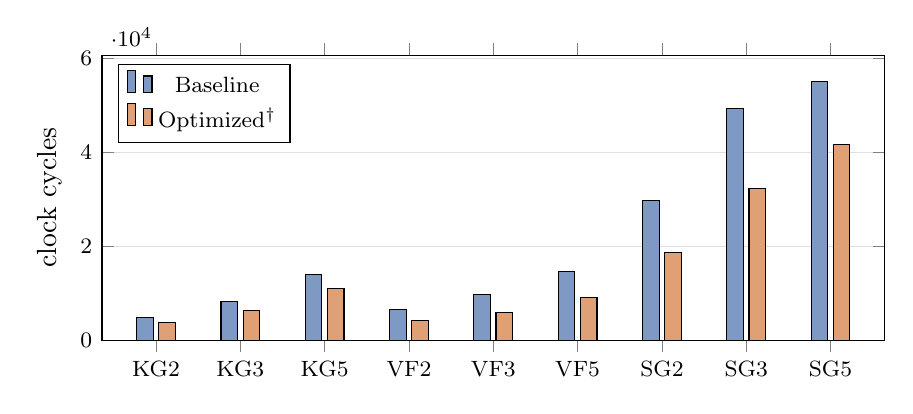
\begin{tikzpicture}
\begin{axis}[ybar,width=0.95\textwidth,height=5.2cm,bar width=6pt,
  symbolic x coords={KG2,KG3,KG5,VF2,VF3,VF5,SG2,SG3,SG5},xtick=data,
  ylabel={clock cycles},ymin=0,legend style={at={(0.02,0.97)},anchor=north west,font=\footnotesize},
  tick label style={font=\footnotesize},enlarge x limits=0.08,ymajorgrids=true,grid style={gray!25}]
\addplot[fill=cA!70] coordinates {(KG2,4875)(KG3,8291)(KG5,14037)(VF2,6582)(VF3,9724)(VF5,14642)(SG2,29795)(SG3,49388)(SG5,55138)};
\addplot[fill=cB!70] coordinates {(KG2,3714)(KG3,6366)(KG5,10980)(VF2,4130)(VF3,5907)(VF5,9063)(SG2,18703)(SG3,32276)(SG5,41742)};
\legend{Baseline,Optimized$^\dagger$}
\end{axis}
\end{tikzpicture}
\caption{Key generation (KG), verification (VF) and expected signing (SG) latency at levels 2, 3, 5.}\label{fig:bars}
\end{figure}

\section{Final Complexity of the Optimized Design}\label{sec:final}
\paragraph{Time.}
Asymptotics are unchanged: $T=\Theta\big(((K{+}L)N\log N+KLN)/P\big)$ per pass and $\mathbb{E}[T_{\text{sign}}]=T_{\text{setup}}+\mathbb{E}[R]\,T_{\text{attempt}}$. What changes are constants: effective parallelism (two operators in key generation and verification, balanced use in signing), the transform cost (300 to about 265 cycles) and the executed fraction of each attempt.

\paragraph{Space.}
Algorithmic space stays $\Theta((KL+K+L)N)$. The runtime build keeps 29 BRAM36; single-level builds fall to about 12, 15 and 24 (O6).

\paragraph{Hardware.}
O5 is the only optimization that removes substantial logic; the others add small control logic. Table~\ref{tab:final-hw} gives the projection.

\begin{table}[H]
\centering
\caption{Projected resources, combined design ($\dagger$). Deltas in LUT/FF: O1 $+$100/$+$50, O2 $+$300/$+$150, O3 $+$400/$+$150, O4 $+$500/$+$150, O5 $-$3\,500/$-$2\,200.}\label{tab:final-hw}
\begin{tabular}{@{}lrrr@{}}
\toprule
Resource & Baseline & Optimized\est & Change\\
\midrule
LUT  & 53\,187 & 50\,000-52\,000 & $\approx-$2 to $-$6\,\%\\
FF   & 28\,318 & 26\,000-27\,500 & $\approx-$3 to $-$8\,\%\\
DSP  & 16 & 16 & 0\\
BRAM36 & 29 & 29 & 0 (single-level: 12-24)\\
\bottomrule
\end{tabular}
\end{table}

The arithmetic datapath is unchanged, so the clock frequency should be too, but this must be confirmed after place and route. Work per LUT improves because the same hardware finishes each operation in 22-39\,\% fewer cycles (except best-case signing).

\section{Limitations and Validity}\label{sec:limits}
\begin{itemize}
  
  \item \textbf{Estimates.} $T_{\text{setup}}$ and $F$ are fitted, so the 0.3\,\% agreement is not independent validation. The 85\,\% factor for O3, the 265-cycle transform of O2 and the area deltas are engineering judgement.
  \item \textbf{Single code reading.} O1 rests on the flag being read only once (Section~\ref{sec:reject}).
  \item \textbf{Level 5} is less certain because its operator assignment differs.
  \item \textbf{Correctness} of any change must be re-established with the 100 KATs per level and the testbenches.
  \item \textbf{Round 3, not FIPS 204.} Results do not transfer directly to ML-DSA.
\end{itemize}

% ======================= 6 =======================
\chapter{Conclusion and Future Work}
% =================================================
\section{Conclusion}
The repository is a well-structured, high-performance FPGA design. Its core is a four-butterfly NTT unit streaming four coefficients per cycle at about 300 cycles per transform, roughly 17\,\% above the ideal 256. Time complexity is $\Theta(N\log N)$ per transform, space is dominated by the matrix $\mathbf{A}$, and area by the Keccak cores, the two operators and UseHint.

The most relevant improvements are in scheduling, not arithmetic: the signing loop does not abort doomed attempts early (O1), and key generation and verification leave the second operator idle (O3). With O2, O4, O5 and O6, expected signing latency is projected to fall by 24-37\,\%, key generation by 22-24\,\% and verification by 37-39\,\%, with LUT and FF use reduced and DSP and BRAM unchanged. Faster Keccak, Montgomery reduction, a wider NTT and a fused multiply-inverse-transform datapath were examined and set aside.

\section{Future Work}
\begin{itemize}
  \item Build the regression harness and run the testbenches in a mixed-language simulator to replace the analytical model with measured stage counts.
  \item Confirm the O1 finding, then implement O1, O3 (with the port-ownership table), O4, O2 and O5, and synthesize to confirm area and frequency.
  \item Verify the baseline tables against the original publication.
  \item Port the optimizations to an ML-DSA (FIPS~204) design, such as the one built on this code base~\cite{norga2026}.
\end{itemize}

% ======================= REFERENCES =======================
\clearpage\phantomsection\addcontentsline{toc}{chapter}{References}
\begingroup\singlespacing\small
\begin{thebibliography}{99}
\bibitem{repo} GMU CERG, \emph{GMUCERG/Dilithium}, GitHub repository, commit f929599, 2022. \url{https://github.com/GMUCERG/Dilithium}
\bibitem{beckwith2021} L.~Beckwith, D.~T.~Nguyen, K.~Gaj, ``High-Performance Hardware Implementation of CRYSTALS-Dilithium,'' \emph{Proc.\ FPT}, 2021; ePrint 2021/1451. \url{https://eprint.iacr.org/2021/1451}
\bibitem{beckwith2022} L.~Beckwith, D.~T.~Nguyen, K.~Gaj, ``High-Performance Hardware Implementation of Lattice-Based Digital Signatures,'' 4th NIST PQC Standardization Conference, 2022. (Source of baseline tables; add URL.)
\bibitem{spec} L.~Ducas et al., ``CRYSTALS-Dilithium: A Lattice-Based Digital Signature Scheme,'' \emph{IACR TCHES}, 2018(1), and Round-3 specification (NIST PQC).
\bibitem{fips204} NIST, ``Module-Lattice-Based Digital Signature Standard,'' FIPS~204, 2024.
\bibitem{fips202} NIST, ``SHA-3 Standard: Permutation-Based Hash and Extendable-Output Functions,'' FIPS~202, 2015.
\bibitem{lyubashevsky2009} V.~Lyubashevsky, ``Fiat-Shamir with Aborts: Applications to Lattice and Factoring-Based Signatures,'' \emph{ASIACRYPT 2009}.
\bibitem{land2021} G.~Land, P.~Sasdrich, T.~G\"uneysu, ``A Hard Crystal - Implementing Dilithium on Reconfigurable Hardware,'' \emph{CARDIS 2021}.
\bibitem{zhao2022} C.~Zhao et al., ``A Compact and High-Performance Hardware Architecture for CRYSTALS-Dilithium,'' \emph{IACR TCHES}, 2022. (Check author list.)
\bibitem{barrett1986} P.~Barrett, ``Implementing the Rivest Shamir and Adleman Public Key Encryption Algorithm on a Standard Digital Signal Processor,'' \emph{CRYPTO '86}, 1987.
\bibitem{montgomery1985} P.~L.~Montgomery, ``Modular Multiplication Without Trial Division,'' \emph{Math.\ Comp.}, 44(170), 1985.
\bibitem{norga2026} Q.~Norga et al., ``ML-DSA-OSH: An Efficient, Open-Source Hardware Implementation of ML-DSA,'' DATE 2026.
\end{thebibliography}
\endgroup

\end{document}